\section{Results}
\label{sec:results}
%
The newly developed code was used to carry out some numerical experiments which are presented in this section.
Aspects that need to be checked are the correctness of the propagators from a quantum mechanical point of view (subsection~\ref{subsec:physical}), convergence of the methods (subsection~\ref{subsec:convergence}) and benchmark of the compute time (subsection~\ref{subsec:benchmark}).
\par\medskip
%
The number of steps $M_{split}$ for the \proc{IntSplit} method can be calculated based on an analysis of the numerical properties of the methods, such that the stability of the propagators is guaranteed.
However, it was found that such an adaptive number of splitting intervals (usually depending on $\Dt$ itself) made the numerical experiments hardly comparable (both in terms of reunite and precision).
Therefore, for all the presented results, $M_{split}=4$ was used for every call to \proc{IntSplit} in order to create fair conditions for comparing the different propagators.
\par\medskip
%
The potentials used for these numerical experiments are the harmonic, torsional and Morse potential that are now briefly introduced.
The semiclassical parameter $\eps = 0.01$ was used if not specified otherwise.


\paragraph{Harmonic Potential} in $D$ dimensions
\begin{align}
	\label{math:harmonic}
	V(\bvec{x}) = \frac{1}{2} \sum_{i=1}^D x_i^2
\end{align}
%
Initial values: $\bvec{q} = (1,\dots,1)^T$, $\bvec{q} = (1,\dots,1,-1,\dots,-1)$, $\bmat{Q}$ and $\bmat{P} = \im \bmat{Q}^{-1}$. \\
\par\medskip


\paragraph{Torsional Potential}
%
\begin{align}
	\label{math:torsional}
	V(\bvec{x}) = \sum_{i=1}^D \left( 1 - \cos x_i \right)
\end{align}
%
Initial values: $\bmat{Q} = \bmat{I}_N$, $\bmat{P} = \im \bmat{I}_N$, $\bvec{q} = (1,0,\dots,0)$, $\bvec{p} = (0,\dots,0)$ (see \cite{FGL_semiclassical_dynamics}).

\paragraph{Morse Potential}
%
\begin{align}
	\label{math:morse}
	V(\bvec{x}) = C e^{-2a(x-x_0)} - 2 e^{-a(x-x_0)} \; .
\end{align}
%
Constants (see \cite{Unpublished}): $C = 0.004164$, $a=0.896696$, $x_0 = 5.542567$. \\
Initial values: $q_0 = 6.0426$, $p_0 = -0.1100$, $Q_0 = 3.4957$, $P_0 = 0.2861 \im$.
The Morse potential was used with $\eps = 0.0484$ for all simulations.


\subsection{Physical Correctness}
\label{subsec:physical}
%
In order to analyze the physical correctness of the implemented propagators, a wave packet was propagated in the various potentials introduced above and the energy conservation was observed.
\par\medskip
%
Figure \ref{fig:energy_Semiclassical} shows the time evolution of energy and the energy drift for the semiclassical propagator. The corresponding energy plots for the remaining propagators can be found in the appendix to the report.
The equivalent conservation plot for the two dimensional case is shown in figure \ref{fig:energy_Semiclassical_2D}.
As is clearly shown by the graphs, the propagators conserve the total energy (except for very small oscillations).
%
\begin{figure}[ht]
	\centering
	\begin{minipage}[c]{\textwidth}
		\begin{center}
			\large Semiclassical Propagator \\[1mm]
			\normalsize Energy Evolution and Drift
			\vspace{4mm}
		\end{center}
	\end{minipage}
	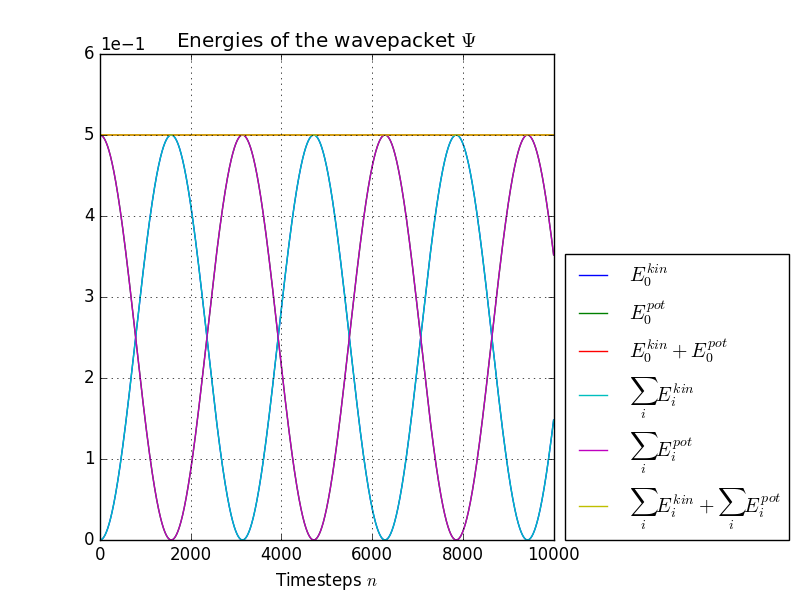
\includegraphics[width=.45\textwidth]{figures/harmonic_1D_Semiclassical_energies.png}
	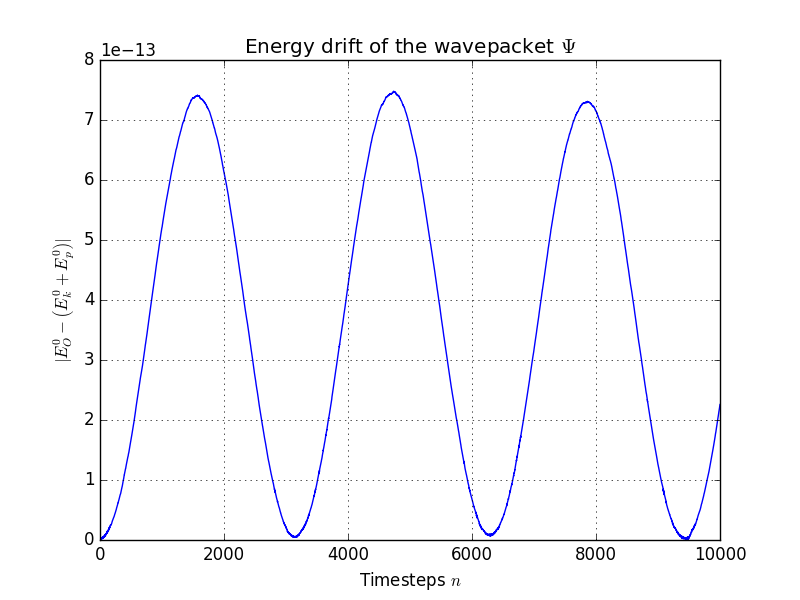
\includegraphics[width=.45\textwidth]{figures/harmonic_1D_Semiclassical_drift.png} \\
	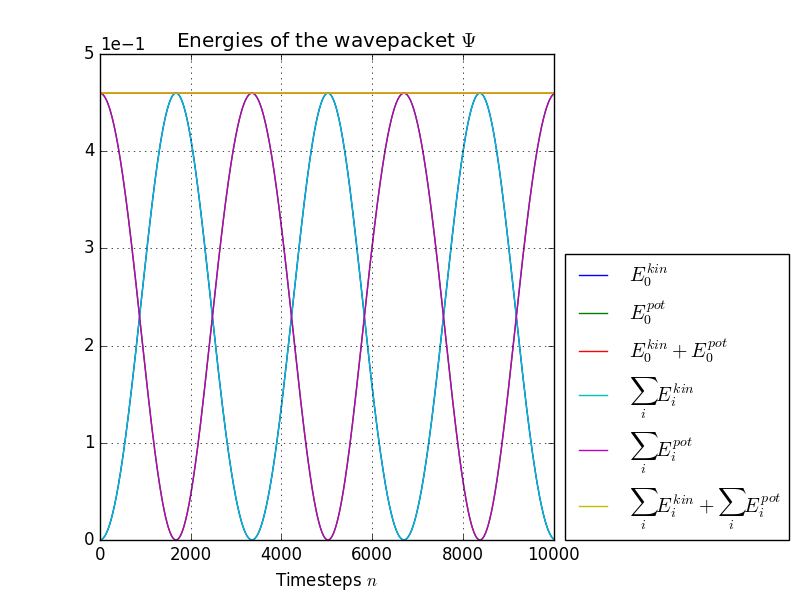
\includegraphics[width=.45\textwidth]{figures/torsional_1D_Semiclassical_energies.png}
	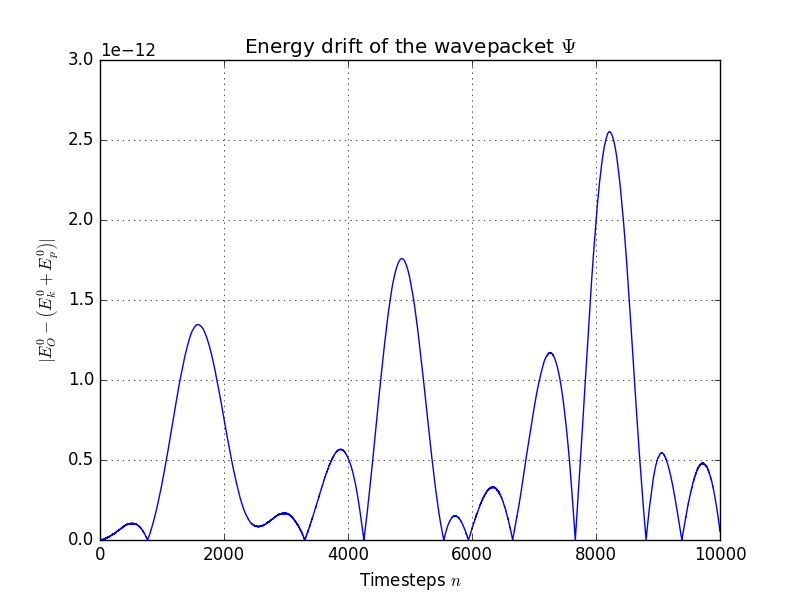
\includegraphics[width=.45\textwidth]{figures/torsional_1D_Semiclassical_drift.png} \\
	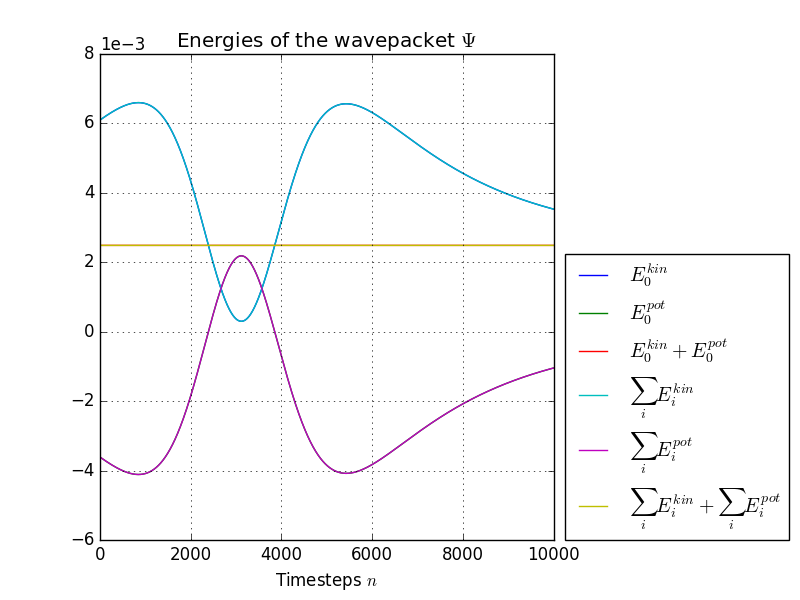
\includegraphics[width=.45\textwidth]{figures/morse_1D_Semiclassical_energies.png}
	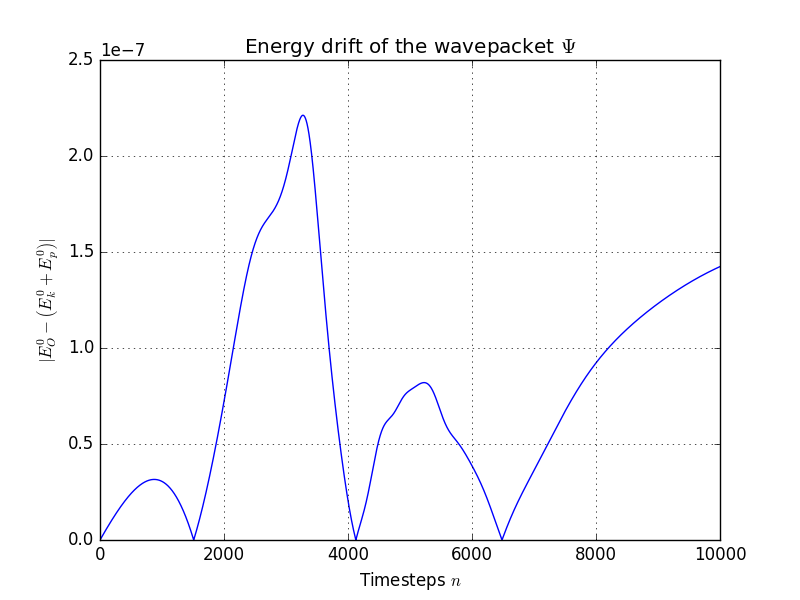
\includegraphics[width=.45\textwidth]{figures/morse_1D_Semiclassical_drift.png}
	\caption{Energy evolution and drift for a 1D wave packet propagated with the Semiclassical propagator in a harmonic potential (top), a torsional potential (middle) and a Morse potential (bottom).
	(Parameters: $N=1$, $D=1$ $|\K|=16$ $\eps=0.01$ (Morse $0.0484$), $T=10$ (Morse $T=50$), $\Dt=0.001$ (Morse $\Dt=0.005$), Semiclassical propagator with \emph{Y4} splitting for \proc{IntSplit})}
	\label{fig:energy_Semiclassical}
\end{figure}
%
\begin{figure}[ht]
	\centering
	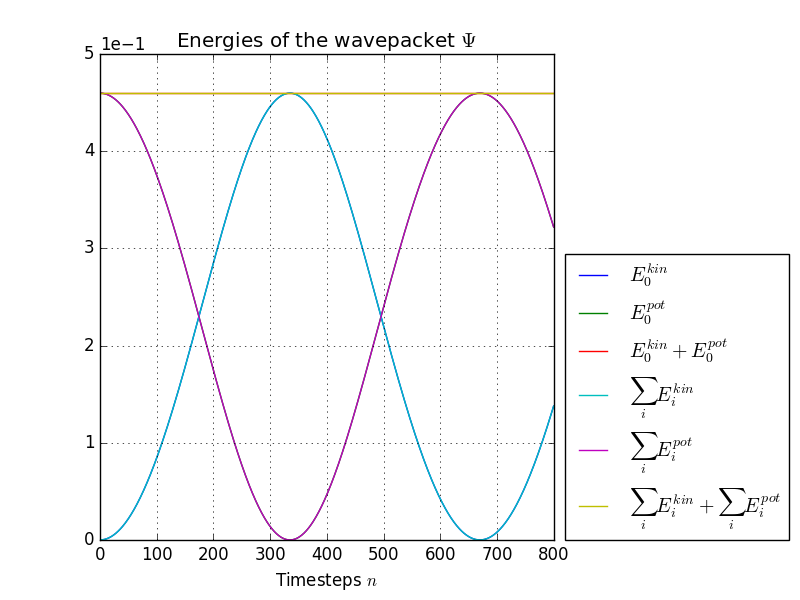
\includegraphics[width=.8\textwidth]{figures/torsional_2D_Semiclassical_energies.png}
	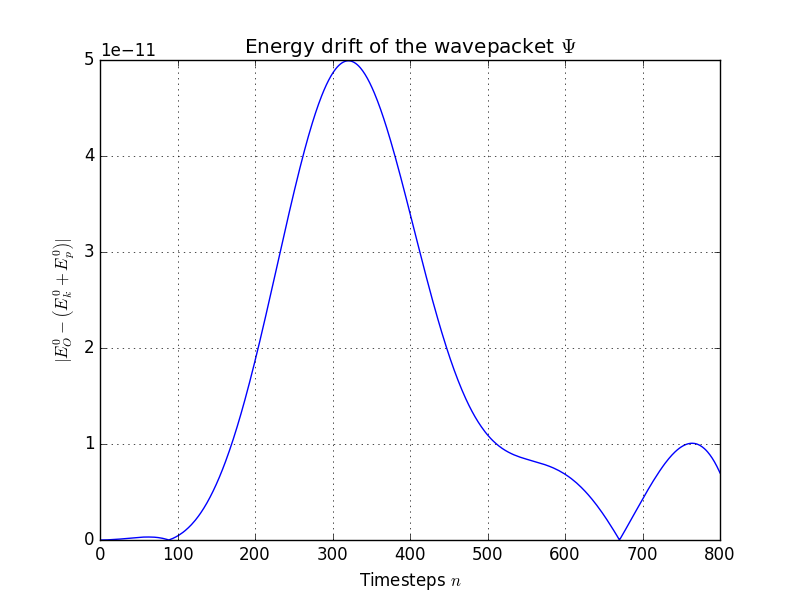
\includegraphics[width=.8\textwidth]{figures/torsional_2D_Semiclassical_drift.png}
	\caption{Energy evolution and drift for a wave packet propagated with the Semiclassical propagator in a 2D torsional potential.
	(Parameters: $N=1$, $D=2$ $|\K|=16$ $\eps=0.01$, $T=4$, $\Dt=0.005$, Semiclassical propagator with \emph{KL10} splitting for \proc{IntSplit})}
	\label{fig:energy_Semiclassical_2D}
\end{figure}


\subsection{Effect of Step size}
\label{subsec:convergence}
%
A convergence analysis was carried out in which the error of each propagator was recorded while reducing the step size $\Dt$.
A \emph{McL84} propagator with \emph{KL10} splitting coefficients and step size $\Dt = 0.0001$ (Morse: $\Dt = 0.0005$) was used to propagate the wave packet to a final time $T = 10$ (Morse: $T=50$) and create a reference solution.
\par\medskip
%
The error between two wave packets was computed by evaluating them on a grid on $[-5,5]$ (Morse: $[0,10]$) with 1000 grid points and taking the $L_2$ norm of the differences.
Figure \ref{fig:error_analysis} shows how the error changes for different step sizes $\Dt$.
All propagators converge towards the reference solution, quickly reaching the limit imposed by the machine precision.
The simplistic Hagedorn propagator shows the largest error and a convergence order of two, similarly to the \emph{Semiclassical} and \emph{McL42} propagators.
The more advanced propagators \emph{MG4}, \emph{McL84} and \emph{Pre764} even show a convergence order of four.
Interestingly enough, if only a \emph{LT} splitting is used in the \proc{IntSplit} method, then the simplistic \emph{Hagedorn} propagator outperforms all the others. However, changing the splitting scheme to \emph{Y4} again gives the expected behavior.
%
\begin{figure}[ht]
	\centering
	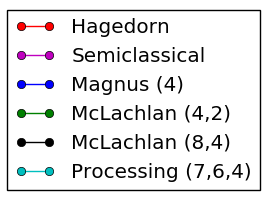
\includegraphics[width=.2\textwidth]{figures/convergence_legend.png} \\
	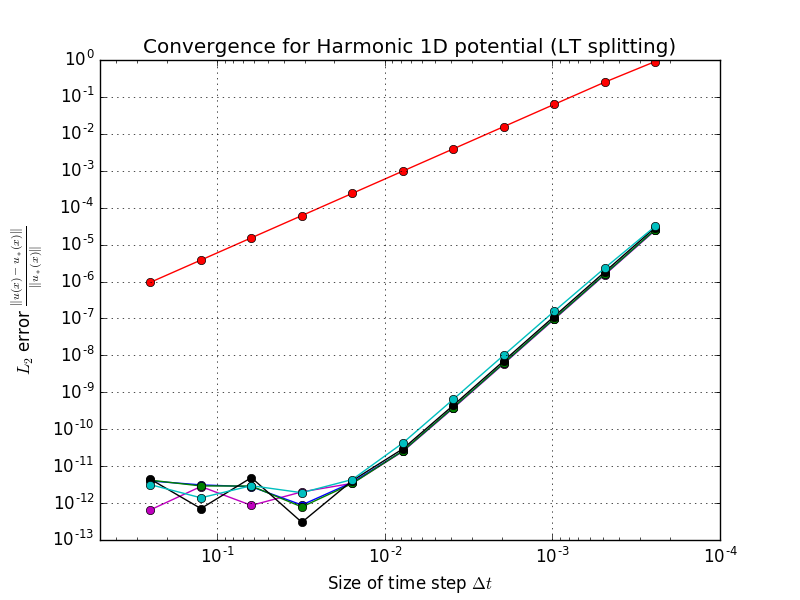
\includegraphics[width=.45\textwidth]{figures/convergence_harmonic_1D_lt.png}
	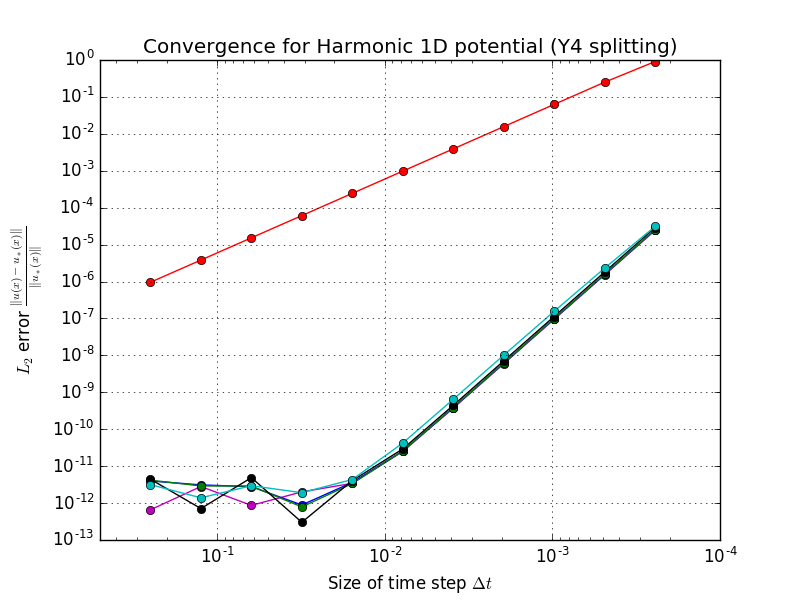
\includegraphics[width=.45\textwidth]{figures/convergence_harmonic_1D_y4.png} \\
	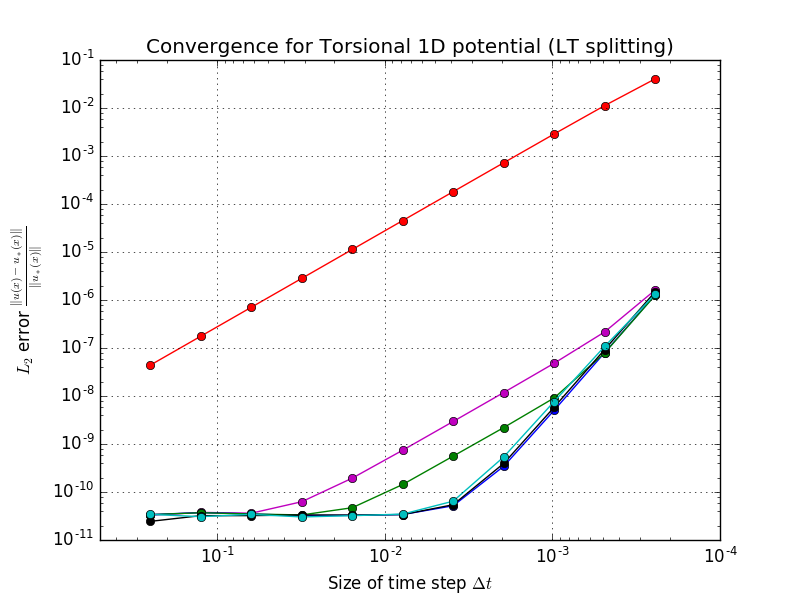
\includegraphics[width=.45\textwidth]{figures/convergence_torsional_1D_lt.png}
	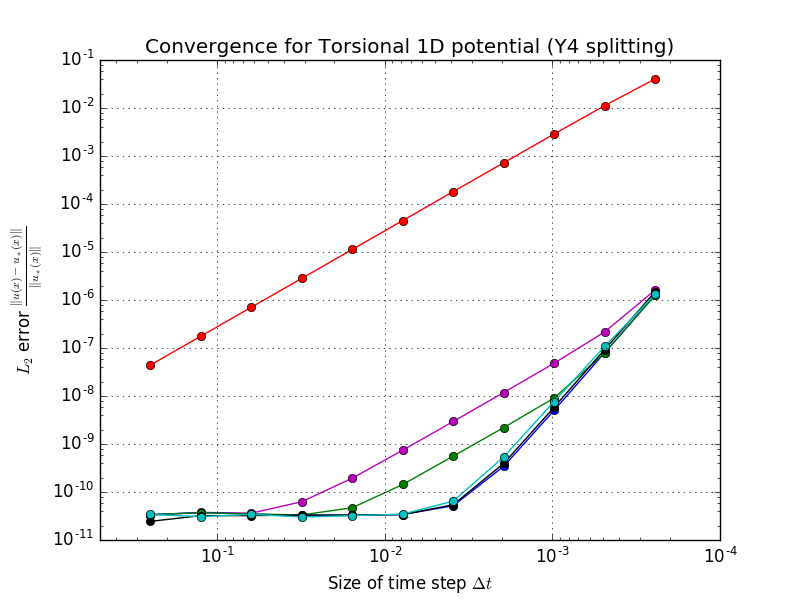
\includegraphics[width=.45\textwidth]{figures/convergence_torsional_1D_y4.png} \\
	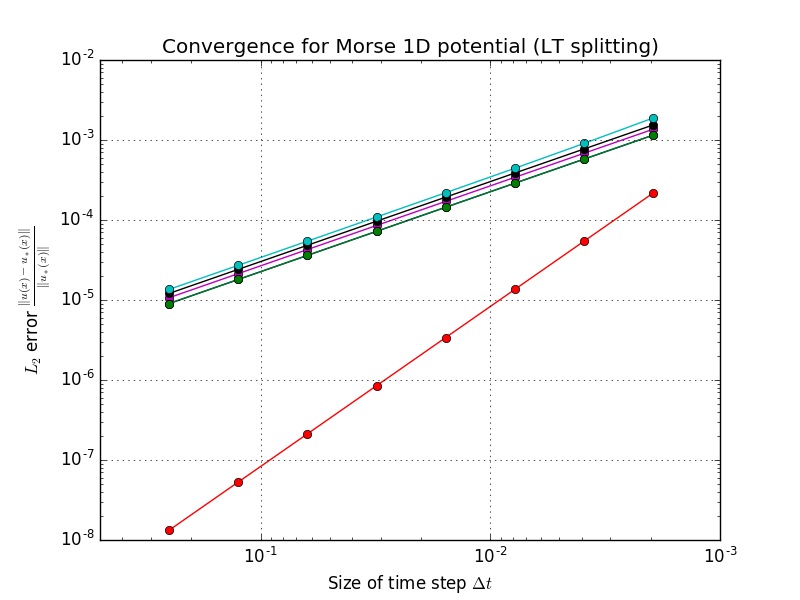
\includegraphics[width=.45\textwidth]{figures/convergence_morse_1D_lt.png}
	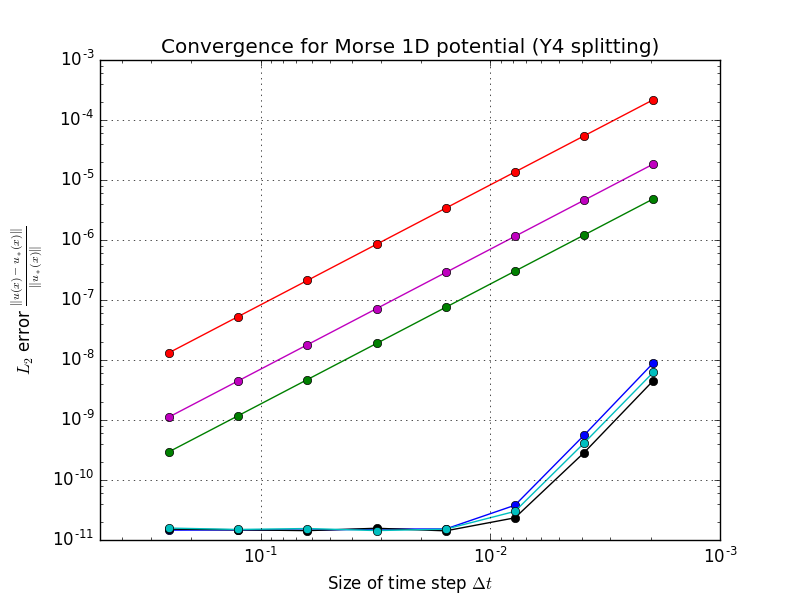
\includegraphics[width=.45\textwidth]{figures/convergence_morse_1D_y4.png}
	\caption{Convergence of the various propagators towards the reference solution for \emph{LT} splitting (left) and \emph{Y4} splitting (right). The potentials are the harmonic potential (top), the torsional potential (middle) and the Morse potential (bottom). The $L_2$ norm was measured by projecting the wave function on a grid with $1000$ nodes in the range $[-5,5]$ (Morse $[0,10]$) and taking the differences of the current solution and the reference solution at $T=10$ (Morse $T=50$).}
	\label{fig:error_analysis}
\end{figure}

\subsection{Benchmark}
\label{subsec:benchmark}
%
In order to benchmark the code, three timing experiments were carried out: a simple comparison of run-times for different propagators, an investigation of the computational cost associated with the usage of high order splitting schemes, and an analysis of the compute time as a function of the dimension $D$.
In all cases, the $1D$ torsional potential introduced at the beginning of this section was used.
\par\medskip
%
The run-time analysis was carried out on a Linux (Kernel 4.8.7, Fedora 24 Workstation) Quad-Core machine with an Intel Core i5-3210M Processor and
4GB of RAM. The C++ code was compiled with the GNU compiler, version 6.2.1, and using the \emph{-Ofast} optimization flag.



\subsubsection{Comparison of propagators}
%
A quick comparison of timings for propagating a wave packet in a 1D torsional potential with different propagators is given in Table~\ref{tab:comparison}.
Surprisingly, the Semiclassical propagator seems to take the same time as the Hagedorn propagator, despite its more complex structure.
The Magnus Propagator \emph{MG4} is cheaper than expected, as it involves two evaluations of $\matrixel{\varphi_k}{W}{\varphi_l}$ per time step but is only slightly slower than the Semiclassical operator with one evaluation of the inner product.
The slowest propagator is \emph{McL84} which involves five propagations with $\opW$ per step.
%
\begin{table}[ht]
	\centering
	\begin{tabular}{|l | r |} 
		\hline
		\multicolumn{1}{|c}{\textbf{Propagator}} &
		\multicolumn{1}{|c|}{\textbf{Timing [s]}} \\
		\hline
		Hagedorn & 27.83 \\
		Semiclassical & 27.66 \\
		MG4 & 37.85 \\
		McL42 & 49.20 \\
		McL84 & 107.62 \\
		Pre764 & 70.93 \\
		\hline
	\end{tabular}
	\caption{Run times for different propagators. The standard deviation of these measurements was below $1\%$.
	(Parameters: torsional potential, $N=1$, $D=1$, $|\K|=16$ $\eps=0.01$, $T=10$, $\Dt=0.0001$, Semiclassical propagator with \emph{Y4} splitting for \proc{IntSplit}) }
	\label{tab:comparison}
\end{table}


\subsubsection{Splitting Schemes}
%
As mentioned previously, the splitting coefficients $\{ w_T, w_U \}$ that are used as weights on the time step $\dt$ in the \proc{IntSplit} method can have vastly different complexity, ranging from the \emph{Lie-Trotter} coefficients (one coefficient for propagation with $\opT$, one for propagation with $\opU$) up to the \emph{KL10} coefficients (34 coefficients for each operator). \\
Higher order schemes are usually preferred in terms of accuracy, but they come at the price of longer computation time.
\par\medskip
%
Therefore, a numerical experiment was carried out in order to analyze how much computational time is required for using different sizes of coefficient pairs $\{ w_T, w_U \}$ in the \proc{IntSplit} method.
The same simulations were carried out for Python and C++ code.
The results are shown in figure \ref{fig:benchmarksplit}.
\par\medskip
%
The Python simulations were run using the Pade matrix exponential, Gauss-Hermite Quadrature, and a \proc{HyperbolicCutShape} as basis shape, while
C++ used the more expensive \proc{HyperCubicShape} as in all other benchmarks.
More information about the different basis shapes can be found in \cite{B_master_thesis}
\par\medskip
%
Looking at the Python timings only, the measurements suggest that in the case of the \emph{KL10} coefficient set, at least 80\% of the total run-time is spend in the \proc{IntSplit} function (since larger coefficient sets $\{ w_T, w_U \}$ only affect the number of steps with operators $\opT$ and $\opU$, but not with operator $\opW$).
\par\medskip
%
When bringing the timings in context with the C++ code, a comparison of absolute run-times is of course not fair since C++ is intrinsically faster than a scripting language like Python and the C++ version has been optimized for speed in many different ways.
However, a very significant result in the context of the work on Propagators is how the speedup increases for larger coefficient pairs.
Using the \emph{KL10} coefficient set instead of a simple \emph{LT} set, the Python code takes more than five times longer.
The same comparison on C++ code shows that in the case of the largest coefficient set \emph{KL10} it doesn't even take twice as long as for the basic \emph{LT} version.
This is a very encouraging result as it means that high order splitting coefficients come at almost no extra cost and the \proc{IntSplit} method was implemented efficiently.
\par\medskip
%
\begin{figure}[ht]
	\centering
	\begin{tabular}{|l | r | r | r | r |} 
		\hline
		\multicolumn{1}{|c}{\textbf{Splitting}} &
		\multicolumn{1}{|c}{\textbf{No. of coefs}} &
		\multicolumn{1}{|c}{\textbf{Python timing [s]}} &
		\multicolumn{1}{|c}{\textbf{C++ timing [s]}} &
		\multicolumn{1}{|c|}{\textbf{Speedup}} \\
		\hline
		LT &1 &47.155 &1.3905 &\textbf{33.91} \\
		S2 &2 &52.934 &1.3817 &\textbf{38.31} \\
		Y4 &4 &65.351 &1.4386 &\textbf{45.42} \\
		PRKS6 &7 &84.075 &1.5122 &\textbf{55.59} \\
		Y61 &8 &90.260 &1.4568 &\textbf{61.96} \\
		KL6 &10 &102.531 &1.6049 &\textbf{63.89} \\
		BM63 &15 &133.415 &1.7763 &\textbf{75.11} \\
		KL8 &18 &151.438 &1.8147 &\textbf{83.45} \\
		KL10 &34 &249.749 &2.2168 &\textbf{112.66} \\
		\hline
	\end{tabular}
	\begin{center}
	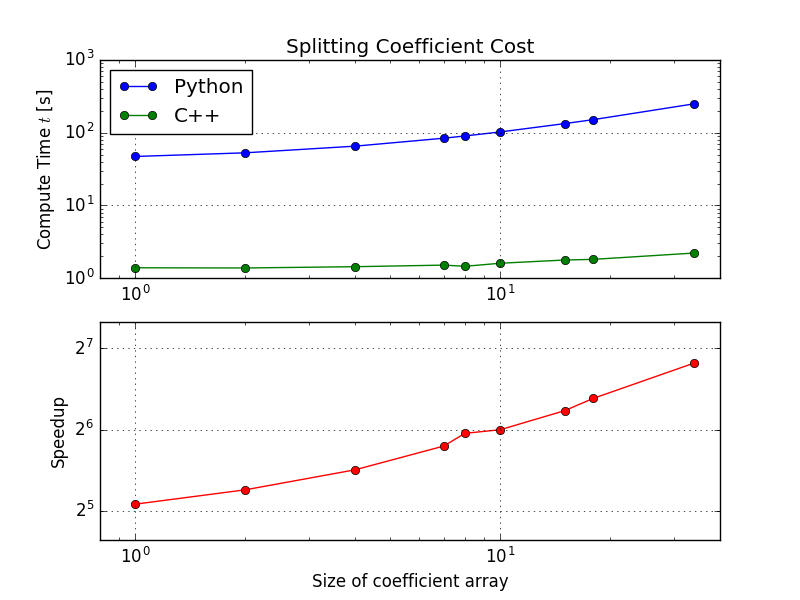
\includegraphics[width=.8\textwidth]{figures/coefs.png}
	\end{center}
	\caption{Comparison of computation times for different splitting coefficients $\{ w_T, w_U \}$ for Python code vs. C++ code. The absolute timings are shown in the top graph, the speedup on the bottom. It is remarkable that the initial speedup factor is about 30, but grows for larger coefficient sets. The speedup factor for the largest tested coefficient pair \emph{KL10} is over 110.
	All the timings in the table were measured by taking the average of 10 independent runs. The standard deviation of these measurements was below $1\%$ for the Python timings and below $0.1\%$ for the C++ timings. (Parameters: $1D$ torsional potential, $N=1$, $|\K|=16$ $\eps=0.01$, $T=10$, $\Dt=0.001$, Semiclassical propagator)}
	\label{fig:benchmarksplit}
\end{figure}


\subsubsection{Scaling with dimensionality D}
%
The question that was addressed in this benchmark is how the compute time of the code scales with increasing dimension $D$ of the wave packet.
Figure \ref{fig:dimension_analysis} shows a clear exponential scaling with the dimension $D$.
With a run-time of just about 35 minutes for 100 time steps with the Semiclassical Propagator, basis size of four and \emph{LT} splitting in $D=5$ dimensions, the computation is still quite feasible.
%
\begin{figure}[ht]
	\centering
	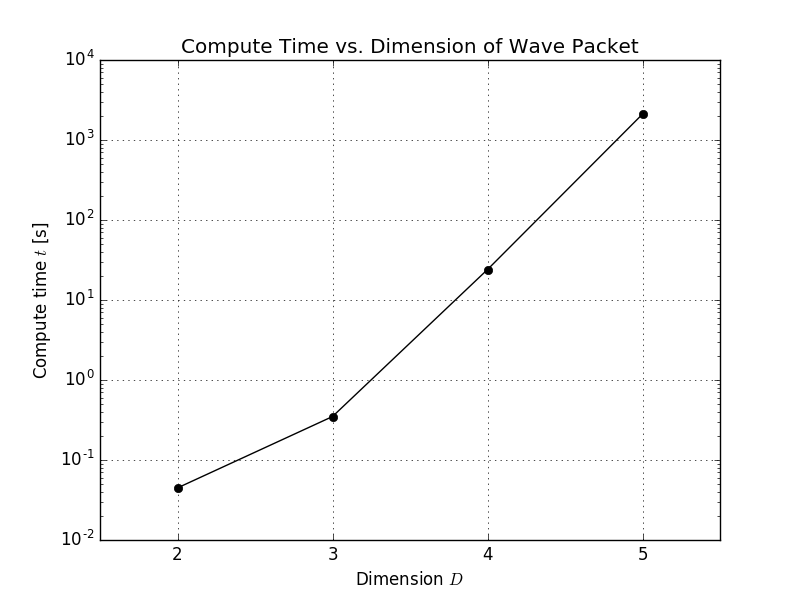
\includegraphics[width=.8\textwidth]{figures/dim.png}
	\caption{Scaling of the computation time with wave packet dimension $D$.
	(Parameters: $D$-dimensional torsional potential, $N=1$, $|\K|=4$ $\eps=0.01$, $T=1$, $\Dt=0.01$, Semiclassical propagator with \emph{LT} splitting for \proc{IntSplit})}
	\label{fig:dimension_analysis}
\end{figure}
